\documentclass[handout,nooutcomes]{ximera}
%% handout
%% space
%% newpage
%% numbers
%% nooutcomes


\renewcommand{\outcome}[1]{\marginpar{\null\vspace{2ex}\scriptsize\framebox{\parbox{0.75in}{\begin{raggedright}P\arabic{problem} Outcome: #1\end{raggedright}}}}}

\renewenvironment{freeResponse}{
\ifhandout\setbox0\vbox\bgroup\else
\begin{trivlist}\item[\hskip \labelsep\bfseries Solution:\hspace{2ex}]
\fi}
{\ifhandout\egroup\else
\end{trivlist}
\fi}

\newcommand{\RR}{\mathbb R}
\renewcommand{\d}{\,d}
\newcommand{\dd}[2][]{\frac{d #1}{d #2}}
\renewcommand{\l}{\ell}
\newcommand{\ddx}{\frac{d}{dx}}
\everymath{\displaystyle}
\newcommand{\dfn}{\textbf}
\newcommand{\eval}[1]{\bigg[ #1 \bigg]}


\title{Breakout Session 4: Reshaping limits}  

\begin{document}
\begin{abstract}
 \textbf{A look back:} In the previous (January 19, 2016) Breakout Session you practiced how to distinguish between the value of a function, the value of a two-sided limit (if it exists), and the value of a one-sided limit (if it exists).

 \textbf{Overview:} In today's (January 21, 2016) Breakout Session you will practice the foundational techniques for computing limits using pen and paper.

  \textbf{A look ahead:} In the next (January 26, 2016) Breakout Session you will investigate how limits are used to formulate vertical and horizontal asymptotes.
\end{abstract}
\maketitle

\section{Learning Outcomes}
\label{section:learning-outcomes}
The following outcomes are \emph{not an exhaustive} list of the skills you will need to develop and integrate for demonstration on quizzes and exams.
This list is meant to be a starting point for conversation (with your Lecturer, Breakout Session Instructor, and fellow learners) for organizing your knowledge and monitoring the development of your skills.
\begin{itemize}
  \item 
    Calculate limits using the limit laws.
  \item 
    Calculate limits of the form $0/0$.
  \item
    Calculate limits of piecewise functions.
  \item 
    Calculate limits using the Squeeze Theorem.
  \item
    Understand what is meant by the form of a limit.
  \item
    Understand the Squeeze Theorem and how it can be used to find limit values.

\end{itemize}
\newpage

\begin{problem}
  \label{problem:identify-application-of-limit-laws}
  The following argument shows 
  \[
    \lim_{x \to 3} \frac{5x^3 - 4 \sqrt{x}}{\sqrt{x^5 - 87}} = \frac{135 - 4\sqrt{3}}{\sqrt{156}}.
  \]
  State which limit law is used to justify each step.
  (A particular step may have more than one limit law as a justification.)

  \begin{align*}
    \lim_{x \to 3} \frac{5x^3 - 4 \sqrt{x}}{\sqrt{x^5 - 87}}
    &= \frac{\lim_{x \to 3} 5x^3 - 4 \sqrt{x}}{\lim_{x \to 3}\sqrt{x^5 - 87}}\\
    &= \frac{5\lim_{x \to 3}(x^3) - 4 \lim_{x \to 3}\sqrt{x}}{\sqrt{\lim_{x \to 3}(x^5 - 87)}}\\
    &= \frac{5(\lim_{x \to 3}x)^3 - 4 \sqrt{3}}{\sqrt{\lim_{x \to 3}(x^5) - \lim_{x \to 3} (87)}}\\
    &= \frac{5(3)^3 - 4 \sqrt{3}}{\sqrt{3^5 - 87}}\\
    &= \frac{135 - 4\sqrt{3}}{\sqrt{156}}
  \end{align*}

  The limits laws:
  
  Assume $\lim_{x \to a} f(x)$ and $\lim_{x \to a} g(x)$ both exist.
  The following properties hold, where $c$ is a real number and $m > 0$ and $n > 0$ are both integers.
  \begin{description}
      \item[1. Sum]
        \[
          \lim_{x \to a} \bigl(f(x) + g(x)\bigr) = \lim_{x \to a} f(x) + \lim_{x \to a} g(x)
        \]

      \item[2. Difference]
        \[
          \lim_{x \to a} \bigl(f(x) - g(x)\bigr) = \lim_{x \to a} f(x) - \lim_{x \to a} g(x)
        \]

      \item[3. Constant multiple]
        \[
          \lim_{x \to a} c \cdot \bigl( f(x) \bigr) = c \cdot \lim_{x \to a} f(x)
        \]

      \item[4. Product]
        \[
          \lim_{x \to a} \bigl(f(x) \cdot g(x)\bigr) = \bigl(\lim_{x \to a} f(x)\bigr) \cdot \bigl(\lim_{x \to a} g(x) \bigr)
        \]

      \item[5. Quotient]
        \[
          \lim_{x \to a} \left(\frac{f(x)}{g(x)}\right) = \frac{\lim_{x \to a} f(x)}{\lim_{x \to a} g(x)},
        \]
        provided $\lim_{x \to a} g(x) \ne 0$

      \item[6. Power]
        \[
          \lim_{x \to a} \bigl(f(x)\bigr)^n = \bigl(\lim_{x \to a} f(x)\bigr)^n
        \]

      \item[7. Fractional power]
        \[
          \lim_{x \to a} \bigl(f(x)\bigr)^{n/m} = \bigl(\lim_{x \to a} f(x)\bigr)^{n/m},
        \]
        provided $f(x) \ge 0$, for $x$ near $a$, if $m$ is even and $n/m$ is reduced to lowest terms
    \end{description}
\end{problem}

\begin{problem}
  \label{problem:evaluating-limits}
  Evaluate each of the following limits analytically using the limit laws.
  \begin{itemize}
    \item[(a)]
      $\displaystyle
        \lim_{x \to 6} \frac{4x^2 - 144}{x-6}
      $
    \item[(b)]
      $\displaystyle
        \lim_{x \to 6} \frac{x-6}{\sqrt{2x-8} - 2}
      $
    \item[(c)]
      $\displaystyle
        \lim_{x \to 2} \frac{(3x-2)^2 - 16}{x-2}
      $
    \item[(d)]
      $\displaystyle
        \lim_{x \to 1} \frac{\sqrt{5x-2} - \sqrt{3}}{x-1}
      $
  \end{itemize}
\end{problem}

\begin{problem}
  \label{problem:evaluating-limit-of-piecewise-function}
  Suppose $f$ is a function defined by
  \[
    f(x) =
    \begin{cases}
      x^2 - ax & \mbox{if $x < 3$}\\
      a2^x + 7 + a & \mbox{if $x > 3$}
    \end{cases}
  \]
  Find $a$ such that $\lim_{x \to 3} f(x)$ exists.
\end{problem}

\begin{problem}
  \label{problem:squeeze-theorem-application}
  For all $x$ near 0 the inequalities $1 - x^2/6 \le \sin(x)/x \le 1$ are true.
  Use these inequalities to find $\displaystyle\lim_{x \to 0} \frac{\sin(x)}{x}$.  
\end{problem}

\begin{problem}
  \label{problem:squeeze-theorem-again}
  Determine the value of $\displaystyle\lim_{x \to 0} x \cos(1/x)$.
\end{problem}

\section{Extra Problem for Personal Practice}
\label{section:extra-problems}
\begin{problem}
  \label{problem:squeeze-theorem-not-trig}
  Determine the value of $\displaystyle\lim_{x \to 0} x^2 \ln(x^2)$.
\end{problem}
% \section*{Warm up:} 
% Below is a table listing all of the Limit Laws, followed by an argument of what the limit of $ \frac{5x^3 - 4 \sqrt{x}}{\sqrt{x^5 - 87}}  $ as $x$ approaches 3 must be.  State which limit law is used to justify each step.

% 	\begin{image}
% 	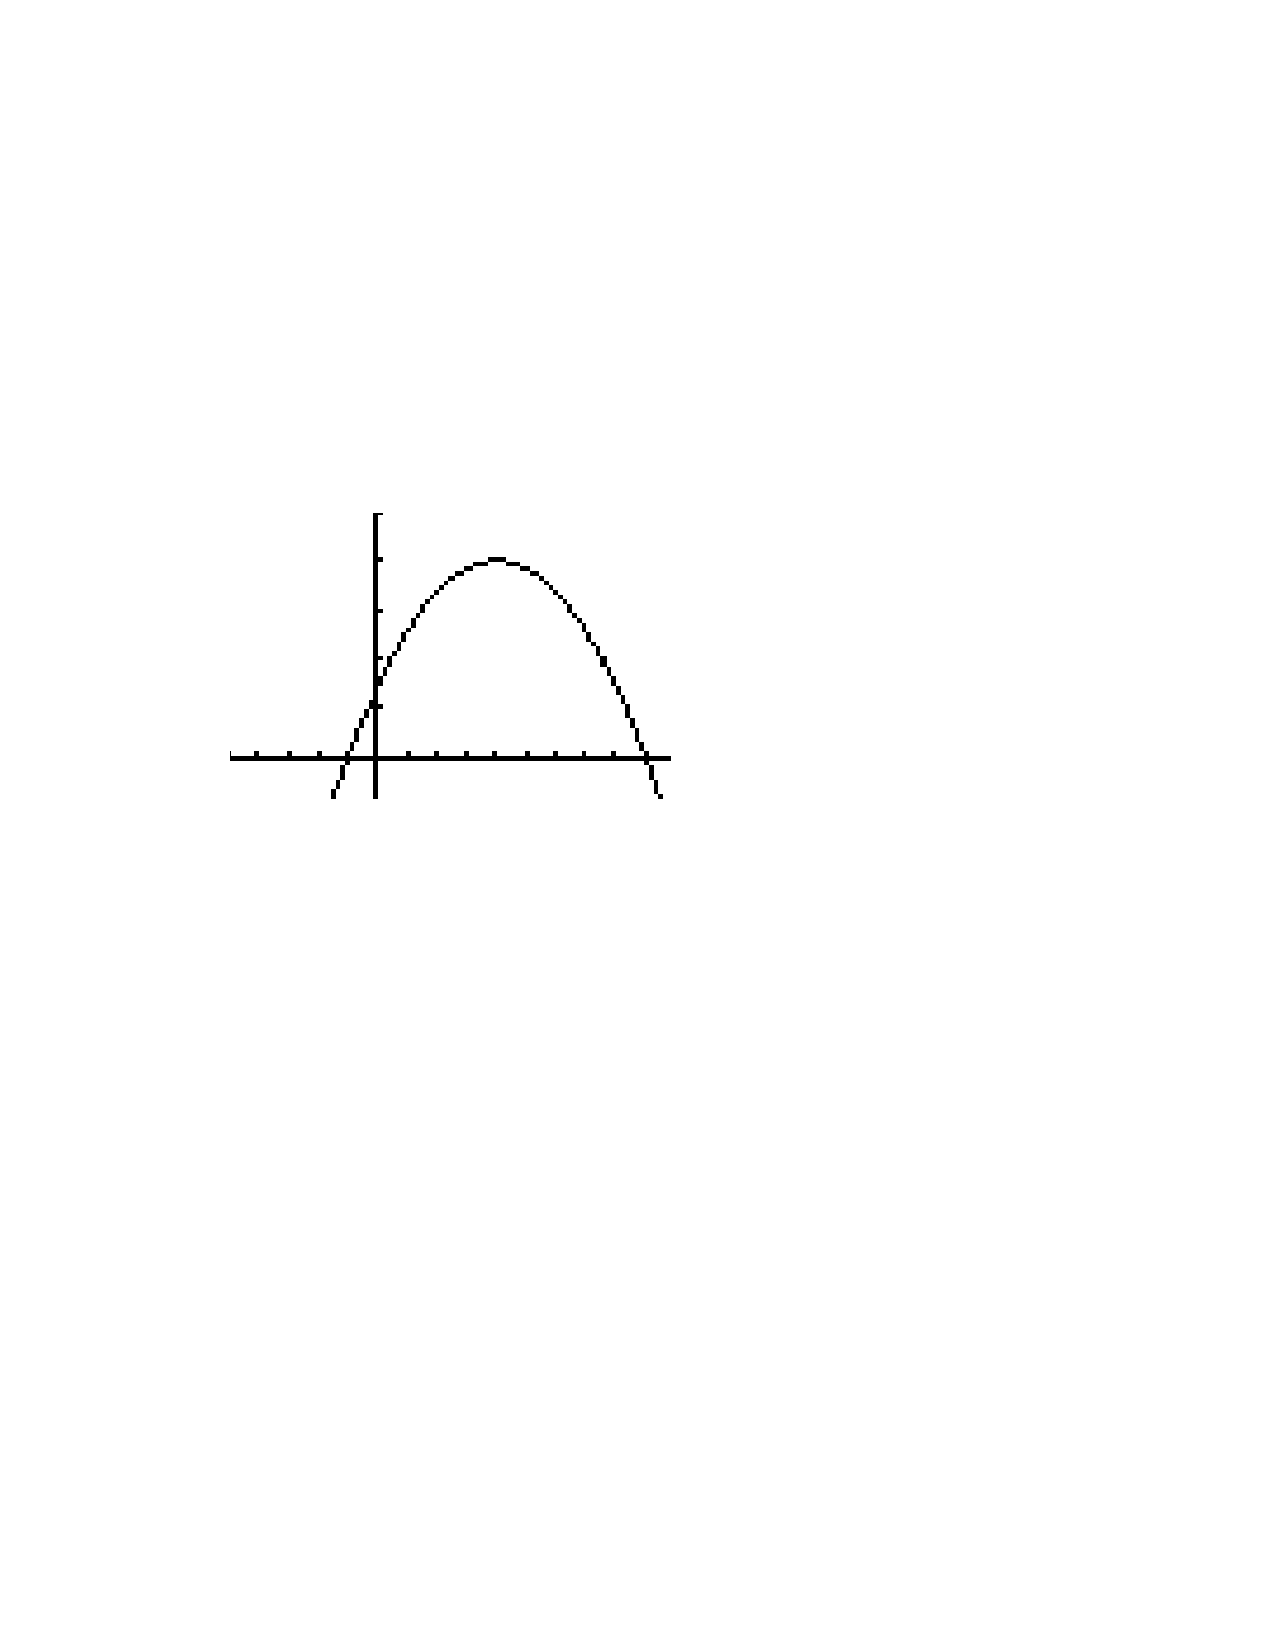
\includegraphics[trim= 250 440 300 175]{Figure1.pdf}
% 	\end{image}

% 	\begin{image}
% 	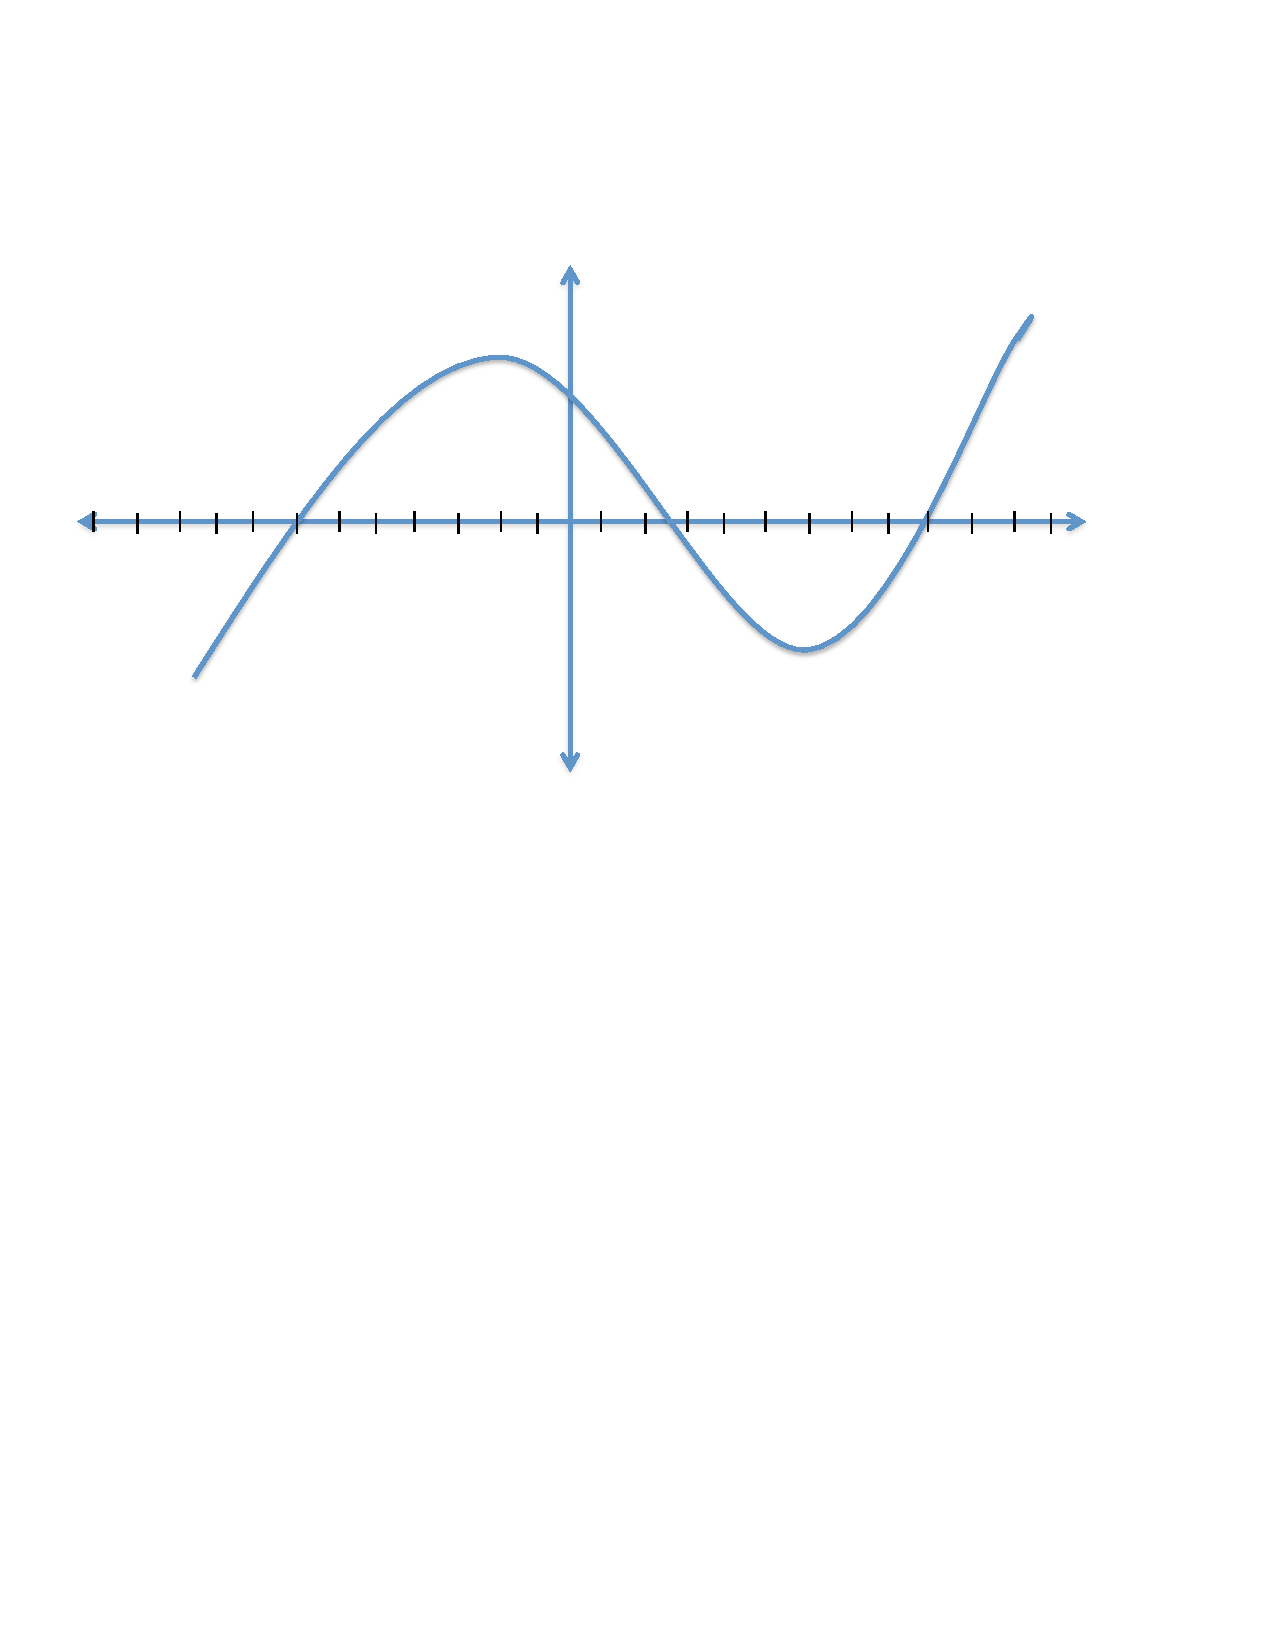
\includegraphics[trim= 150 440 300 185]{Figure2.pdf}
% 	\end{image}
% \newpage
% 	\begin{freeResponse}
% 	Step 1:  Limit law 5.
		
% 	Step 2:  Limit laws 2 and 3 in the numerator, limit law 7 in the denominator.
		
% 	Step 3:  In the numerator both limit law 6 as well as the fact that $\lim_{x \to a}x = a$ are used.  Limit law 2 is used in the denominator.
		
% 	Step 4:  $\lim_{x \to a}x = a$ is used in the numerator.  This same fact, in conjunction with limit law 6, is used in the denominator.
		
% 	Step 5:  This step is just arithmetic.
% 	\end{freeResponse}
	
	

% \section*{Group work:}

% %problem 1
% \begin{problem}
% Evaluate the following limits algebraically using the limit laws.  
	
% 	\begin{enumerate}
	
% 	%part a		
% 	\item $ \lim_{x \to 6} \frac{4x^2 - 144}{x-6}  $
% 	\begin{freeResponse}
% 	\begin{align*}
% 	\lim_{x \to 6} \frac{4x^2 - 144}{x-6} &= \lim_{x \to 6} \frac{4(x-6)(x+6)}{x-6} \\
% 	&= \lim_{x \to 6} 4(x+6) \\
% 	&= 4(12) = 48  
% 	\end{align*}
% 	\end{freeResponse}
	
	
% 	%part b		
% 	\item  $ \lim_{x \to 6} \frac{x-6}{\sqrt{2x-8} - 2}  $
% 	\begin{freeResponse}
% 	\begin{align*}
% 	\lim_{x \to 6} \frac{x-6}{\sqrt{2x-8} - 2} &= \lim_{x \to 6} \frac{x-6}{\sqrt{2x-8} - 2} \cdot \frac{\sqrt{2x-8} + 2}{\sqrt{2x-8}+2} \\
% 	&= \lim_{x \to 6} \frac{(x-6)(\sqrt{2x-8} + 2)}{2x - 8 - 4} \\
% 	&= \lim_{x \to 6} \frac{(x-6)(\sqrt{2x-8} + 2)}{2(x-6)} \\
% 	&= \lim_{x \to 6} \frac{\sqrt{2x-8}+2}{2} \\
% 	&= \frac{\sqrt{12-8}+2}{2} \\
% 	&= \frac{4}{2} = 2
% 	\end{align*}
			
% 	\end{freeResponse}
	
	
% 	%part c		
% 	\item  $ \lim_{x \to 2} \frac{(3x-2)^2 - 16}{x-2}  $
% 	\begin{freeResponse}
% 	\begin{align*}
% 	\lim_{x \to 2} \frac{(3x-2)^2-16}{x-2} &=\lim_{x \to 2} \frac{((3x-2)-4)((3x-2)+4)}{x-2} \\
% 	&= \lim_{x \to 2} \frac{(3x-6)(3x+2)}{x-2} \\
% 	&= \lim_{x \to 2} \frac{3(x-2)(3x+2)}{x-2} \\
% 	&= \lim_{x \to 2} 3(3x+2)  \\
% 	&= 3(6+2) = 24   
% 	\end{align*}
% 	\end{freeResponse}
	
	
% 	%part d		
% 	\item  $ \lim_{x \to 1} \frac{\sqrt{5x-2} - \sqrt{3}}{x-1} $
% 	\begin{freeResponse}
% 	\begin{align*}
% 	\lim_{x \to 1} \frac{\sqrt{5x-2} - \sqrt{3}}{x-1} &= \lim_{x \to 1} \frac{\sqrt{5x-2} - \sqrt{3}}{x-1} \cdot \frac{\sqrt{5x-2} + \sqrt{3}}{\sqrt{5x-2} + \sqrt{3}} \\
% 	&= \lim_{x \to 1} \frac{(5x-2)-3}{(x-1)(\sqrt{5x-2} + \sqrt{3})} \\
% 	&= \lim_{x \to 1} \frac{5(x-1)}{(x-1)(\sqrt{5x-2} + \sqrt{3})} \\
% 	&= \lim_{x \to 1} \frac{5}{\sqrt{5x-2} + \sqrt{3}} \\
% 	&=   \frac{5}{\sqrt{5(1)-2} + \sqrt{3}} \\
% 	&= \frac{5}{2 \sqrt{3}} 
% 	\end{align*}
% 	\end{freeResponse}
% 	\end{enumerate}
% \end{problem}
	
	
	
	
			
			

% %problem 2			
% \begin{problem}
% Suppose
% 	$f(x) =   \left\{ \begin{array}{lr}
% 	x^2 - ax 	&	\text{if } x < 3	\\
% 	a2^x + 7 + a	&	\text{if } x > 3	\end{array} \right.  $
	
% 	Find $a$ so that $ \lim_{x \to 3} f(x)  $ exists.
% 	\begin{freeResponse}
% 	 We need to find $a$ so that $\lim_{x \to 3^-} f(x) = \lim_{x \to 3^+} f(x) $.  
	
% 	\begin{itemize}
	
% 	\item  $\lim_{x \to 3^-} f(x) = \lim_{x \to 3^-} (x^2 - ax) = 9 - 3a $.
	
% 	\item  $\lim_{x \to 3^+} f(x) = \lim_{x \to 3^+} a2^x + 7 + a = a2^3 + 7 + a = 9a + 7 $
	
% 	\end{itemize}
	
% 	So we want $a$ to be such that:
% 	$$ 9-3a = 9a+7 $$
% 	$$12a = 2 $$
% 	$$a = \frac{1}{6}   $$
% 	\end{freeResponse}
% \end{problem}
	
	
	
	
	
	
	
	
	
% %problem 3	
% \begin{problem}
% Sketch the graph of a function with the given properties.  You need not find a formula for the function:
	
% 	$ f(3) = -2, f(-2) = 3, f(5) = 6, \lim_{x \to 5^-} f(x) = -1, \lim_{x \to 5^+} f(x) = 4, \lim_{x \to 3} f(x) = 7  $
	
% 	$ \lim_{x \to -2^-} f(x) = 3, \lim_{x \to -2^+} f(x) = 0, \lim_{x \to 1^+} f(x) = 5  $
	
% 	\begin{freeResponse}
% 	There exist infinitely many functions whose graph satisfies the conditions above, but one such graph is the following:
	
% \newpage
	
% 		\begin{image}
% 		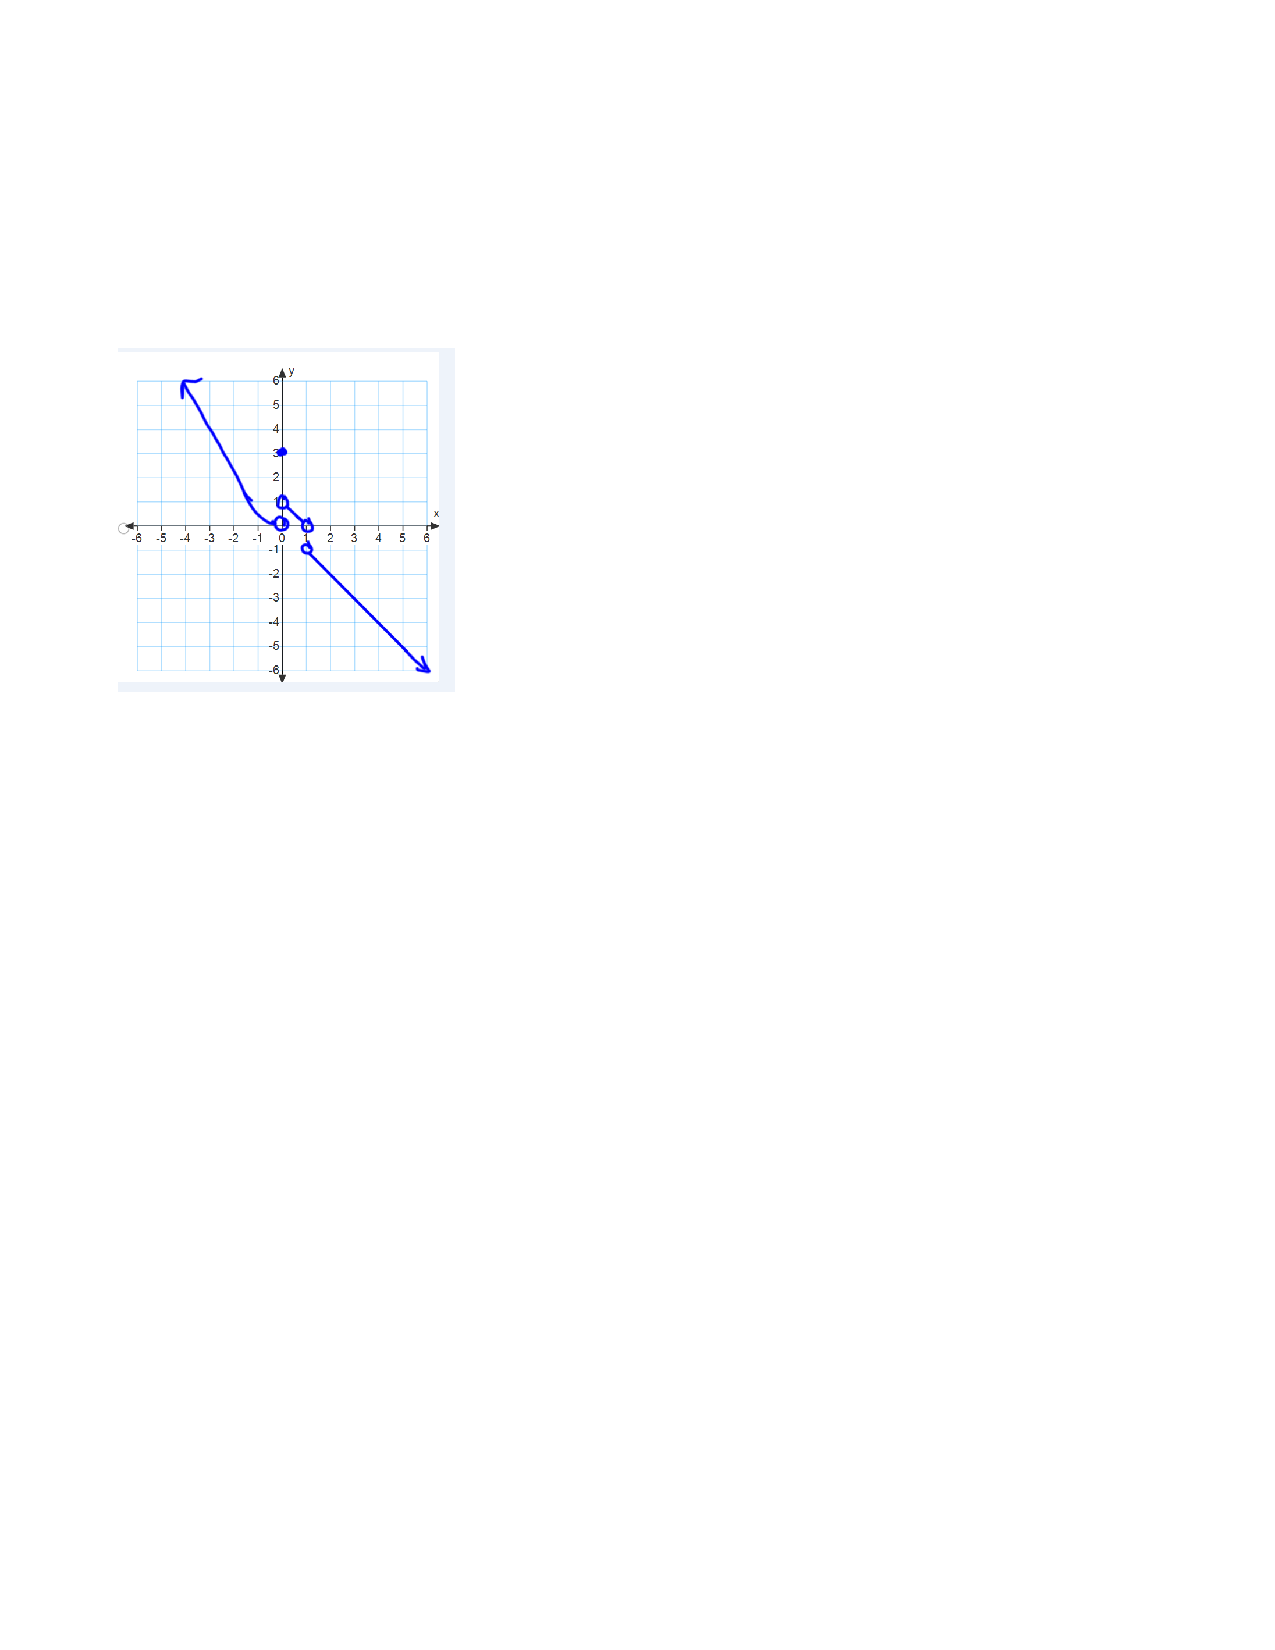
\includegraphics[trim= 450 620 10 0]{Figure3.pdf}
% 		\end{image}
% 	\end{freeResponse}
% \end{problem}
\end{document} 
